\begin{refsection}

\chapter{Scaling sequence library multiplexing with semi-automated liquid handling}

\chapterauthor{Russell Y. Neches, Mary Huang}

\section{Abstract}

You have a couple of thousand of raw samples that need to be diluted to a standard concentration. You don't have a liquid handling robot, but you do have a plate reader, a 3D printer and a multichannel pipetter. Measure your sample concentrations on the plate reader, and put them in a CSV file. Load the CSV file into the web app, and enter the desired concentration. The app will generate a 3D printable plate with custom volumes. Print the model (it will print as a single surface shell, suitable for spiralized printing), and fill all of the wells with buffer. Remove 100 \si{\micro\liter} from each well with the multichannel pipetter, and then transfer the specified volume of your raw samples into the corresponding wells on the dilution plate. The samples will then be at the desired concentration. Dilution ratios among the samples must be within about a factor of 100 of one another.

\section{Materials \& Methods}

\begin{figure}
    \centering
    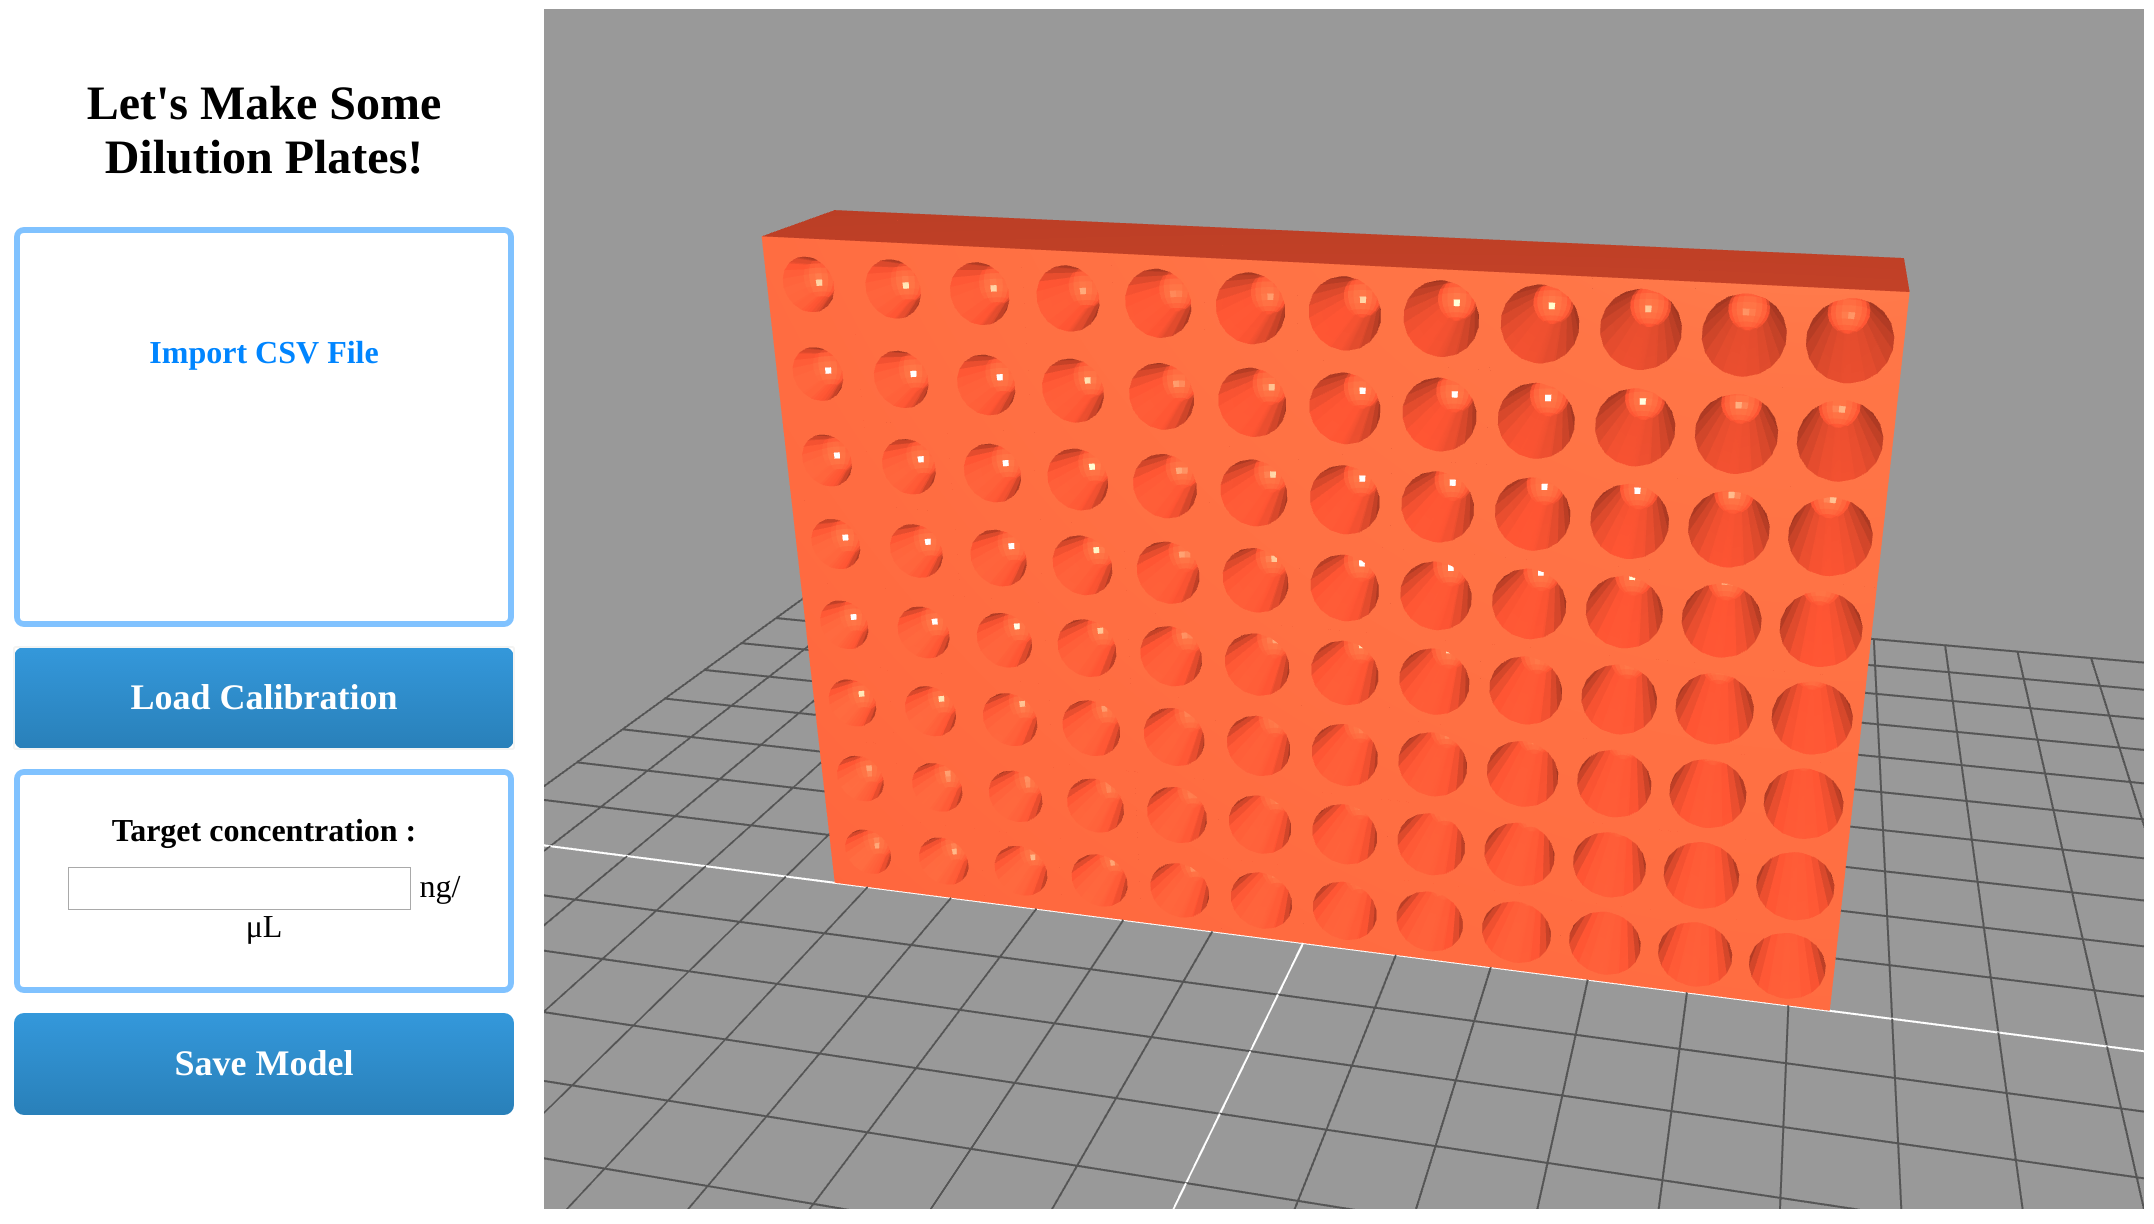
\includegraphics[width=\textwidth]{DilutionPlates/figures/fig1}
    \caption{\textbf{Prototype {\tt DilutionPlates} web applicaiton.}}
    \label{DP_fig1}
\end{figure}

\section{Discussion}

In 2014, our lab produced a sequencing run that yielded 41.7 billion base pairs of data at the cost of \$2,346. The project in question targeted an organism with a large ($>800$ megabase) genome, and so it achieved a coverage of about $50\times$. Most bacteria and archaea have genomes between one and ten megabases. In principle, it should be possible to multiplex hundred, or perhaps thousands, of isolate genomes into a single high-throughput sequencing run. For smaller entities, such as amplicons, viruses, plasmids or synthetic constructs, modern sequencing platforms have the capacity to process hundreds of thousands or millions of multiplexed samples. The reality, unfortunately, is that there are impediments to scaling a multiplexed run to this extent, resulting in wasted sequencing capacity and missed scientific opportunities.

The first bottleneck is DNA extraction. The DNA extraction kits on which many fields, such as microbial ecology, have standardized cost between \$1 and \$10 per sample. Including controls, a project with 470 multiplexed samples using PowerSoil kit\footnote{(The 96-well format version of the Qiagen DNeasy PowerSoil kit costs \$5 per sample :\\ \url{https://www.qiagen.com/us/shop/sample-technologies/dna/dna-preparation/dneasy-powersoil-htp-96-kit/}} would have to budget more money for DNA extraction than sequencing. For many projects, the DNA extraction bottleneck can be avoided by substituting in-house protocols for kit-based protocols, or by selecting downstream steps that are compatible with raw cell lysate or supernatent.

The second bottleneck is barcoding. At high concentration, oligos for sequencing and barcoding cost between \$9.25 \$100 each.\footnote{Assuming \$0.37 per base pair and 25 base pairs at 250 \si{\nano\mole} DNA at the low end, or \$2 per base pair and 50 base pairs at 1 \si{\micro\mole} DNA at the high end.} Oligo synthesis costs will exceed sequencing costs somewehere between 23 and 93 samples, though oligos can be used for many sequencing runs. If one were to spend an equal amount on PowerSoil DNA extraction kits and sequencing, the oligos for 470 samples would cost at least \$4,347, double the cost of sequencing. Without reagents or labor, sequencing would make up only a quarter of the project cost. The solution to this problem is combinatoric barcoding; barcodes are attached to either end of the sequenced fragments, allowing unique combinations of barcoades to uniquely identify samples. With this approach, the number of oligos required scales with the square root of the number of samples required. For 470 samples, 22 oligos would be required, at a cost of at least \$203 (the worst case, \$2,200, is slightly less than the sequencing cost).

The third bottleneck is labor. Obviously, projects with more samples will involve more basic operations. However, to understand how this impedes large-scale multiplexing, it is important to examine in detail what changes about the work as the number of samples increases dramatically. As an example, let us consider a project that uses transposon-based tagmentation \cite{adey2010rapid} to sequence a large number of genomes from bacterial isolate cultures. The tagmentation process is robust enough to function on ``dirty'' DNA, and so we use the supernatent of heat-treated lysate instead of a DNA extraction kit. Here is a schematic protocol for preparing genomic libraries :

\begin{itemize}[noitemsep]
\item \textbf{aliquot samples into bead-beating plates}
\item bead beat samples
\item incubate
\item centrifuge lysate
\item aliquot supernatent to clear bottom plates
\item quantify DNA concentration on plate reader
\item calculate dilution ratio to normalize all samples
\item \textbf{pipette buffer into reaction plates}
\item \textbf{pipette sample into reaction plates}
\item aliquot oligos
\item aliquot reagents
\item incubate
\item heat kill reagents
\item combine samples into multiplexed library
\item quantify and normalize library
\item sequence
\end{itemize}

\noindent The steps that require treating each sample individually are in bold. The first such step is sample intake, which is unavoidable, and many laboratories have straightforward procedures to optimize sample intake using standardization and parallelization. Citizen science projects may reduce this burden with protocols that shift some of the burden of sample intake to the larger group (for example, by using pre-indexed plates and a web-based registration process). 

The second two steps, in which the DNA yielded from each sample is diluted to a standard concentration, scale linearly with the number of samples. For every sample, the operator must perform at least thirteen separate operations :

\subfile{DilutionPlates/table1}

\noindent This assumes the operator does not change tips for the pipetter used for buffer, which may be poor practice. When I have timed myself, 


\printbibliography[heading=subbibliography]

\end{refsection}